% Supplementary material -- separate entry point.
% Build: tectonic supplementary.tex
\documentclass[10pt,twocolumn,letterpaper]{article}

\usepackage[review]{cvpr}
%% Preamble for the FastVCL CVPR draft.
%% The document class and cvpr.sty are loaded in main.tex; this file only adds
%% packages, math macros and the visible TODO marker.

% ---------------------------------------------------------------------------
% Layout / tables / algorithms
% ---------------------------------------------------------------------------
\usepackage{array}
\usepackage{multirow}
\usepackage{tabularx}
\usepackage{algorithm}
\usepackage{algpseudocode}
\usepackage{enumitem}
\usepackage{amsthm}

% Algorithm floats inside the two-column text
\renewcommand{\algorithmicrequire}{\textbf{Input:}}
\renewcommand{\algorithmicensure}{\textbf{Output:}}
\floatname{algorithm}{Algorithm}

% Slightly tighter lists
\setlist[itemize]{leftmargin=1.2em,topsep=2pt,itemsep=1pt,parsep=0pt}
\setlist[enumerate]{leftmargin=1.5em,topsep=2pt,itemsep=1pt,parsep=0pt}

% ---------------------------------------------------------------------------
% Visible placeholders.  DO NOT redefine these to be empty: an empty TODO would
% make the draft look finished while the evidence is still outstanding.
% ---------------------------------------------------------------------------
\newcommand{\red}[1]{{\color{red}#1}}
\newcommand{\todo}[1]{{\color{red}#1}}
\newcommand{\TODO}[1]{\textbf{\color{red}[TODO: #1]}}
\newcommand{\PENDING}{\TODO{PENDING}}
\newcommand{\pending}{--}

% ---------------------------------------------------------------------------
% Math notation
% ---------------------------------------------------------------------------
\newcommand{\fA}[1]{\bar{f}^{A}_{#1}}
\newcommand{\fB}[1]{\bar{f}^{B}_{#1}}
\newcommand{\Sim}{S}
\newcommand{\Tube}{\mathcal{T}}
\newcommand{\Anch}{\mathcal{A}}
\newcommand{\Grid}{\mathcal{G}}
\newcommand{\Pred}{\mathcal{P}}
\newcommand{\Step}{\mathcal{S}}
\newcommand{\Track}{\mathcal{I}}
\newcommand{\TopK}{\operatorname{TopK}}
\newcommand{\Dedup}{\operatorname{Dedup}}
\newcommand{\AnchorCap}{\operatorname{Cap}}
\newcommand{\minIoU}{\operatorname{IoU}_{\min}}
\newcommand{\IoU}{\operatorname{IoU}}
\newcommand{\Tloc}{T_{\mathrm{localize}}}
\newcommand{\Taug}{T_{\mathrm{aug}}}
\DeclareMathOperator*{\argmax}{arg\,max}
\DeclareMathOperator*{\argmin}{arg\,min}

% Shorthand for the two video labels (never use them as a batch size)
\newcommand{\vidA}{\mathrm{A}}
\newcommand{\vidB}{\mathrm{B}}

% ---------------------------------------------------------------------------
% Small spacing helpers
% ---------------------------------------------------------------------------
\newcommand{\tabnote}[1]{\par\vspace{-2pt}{\footnotesize #1}}
\setlength{\abovedisplayskip}{4pt}
\setlength{\belowdisplayskip}{4pt}
\setlength{\abovedisplayshortskip}{2pt}
\setlength{\belowdisplayshortskip}{2pt}


\definecolor{cvprblue}{rgb}{0.21,0.49,0.74}
\usepackage[breaklinks,colorlinks,allcolors=cvprblue]{hyperref}

\def\paperID{*****}
\def\confName{CVPR}
\def\confYear{2027}

\title{Supplementary Material for FastVCL: Training-Free Sparse-to-Tube Video Copy Localization}
\author{Anonymous submission\\Paper ID \paperID}

\begin{document}
\maketitle

\section{Scope and evidence grades}
\label{sec:s-scope}

This supplement records what was verified, what is proposed, and what is still missing. It is
not an extra results section. The grades are:
\textsc{source-verified} (checked against a paper or code location),
\textsc{proposed} (specified but not validated),
\textsc{implemented-unvalidated} (present in the reference implementation, not established
as beneficial), \textsc{pilot-only} (small or incomplete development run),
\textsc{missing}, and \textsc{conflict}. No claim in the main paper or this supplement is
benchmark-verified for FastVCL.

\section{Hyperparameters of the reference configuration}
\label{sec:s-hyper}

The values below are development initial values, not tuned results. Changing them is part of
E2/E4, not of the definition of the method.

\begin{table}[h]
\centering
\caption{Reference configuration (feature-index units unless noted).}
\label{tab:s-hyper}
\footnotesize
\setlength{\tabcolsep}{3pt}
\begin{tabular}{@{}l l@{}}
\toprule
Group & Value \\
\midrule
Sampling & stride 4; Top-$K$ 1; $\tau=0.7$; mutual on \\
         & multi-scale off; independent phases off \\
         & anchor cap 20,000; chunk 64 MB / 512 rows \\
RANSAC   & $\epsilon_B=4.0$; $h_{\min}=5$; max tracks 8 \\
         & $g_A=g_B=24$; $g_{\mathrm{back}}=1.0$ \\
         & $L^A_{\min}=4$; $L^B_{\min}=8$ \\
         & slope $[0.5,2.0]$; 2,000 iterations; conf.\ 0.99 \\
         & unweighted least squares; refit on \\
Tube     & $w_r=12$; $e_A=16$; prototype margin 2 \\
         & min durations $3$ (A), $4$ (B); min anchors 2 \\
         & $\tau_{\mathrm{align}}=0.6$; $\lambda_{\mathrm{gap}}=0.1$ \\
         & smoothing window 3; max 4 paths per tube \\
         & low-quality gap $g_{\mathrm{low}}=2$; $\theta_{\mathrm{dedup}}=0.8$ \\
         & max 64 segments per pair \\
Runtime  & CPU/NumPy; float32 similarity; float64 DP \\
         & per-tile profiling disabled for timing \\
\bottomrule
\end{tabular}
\end{table}

\section{Sampling properties and span bound}
\label{sec:s-sampling}

\paragraph{Nested grids.} With zero phases, a stride-8 grid samples a subset of stride 4,
which samples a subset of stride 2. A coarser plan therefore adds no coordinate but changes
each row's Top-$K$ competition and adds arithmetic. For $64\times64$ inputs, one direction
has $32^2=1{,}024$ grid pairs at stride 2 and $32^2+16^2+8^2=1{,}344$ for $\{2,4,8\}$. The
two are not equal-budget controls; both directions and tie rescans are additional.

\paragraph{Independent phases.} A synchronous shift $(p,p)$ only covers offsets with
$p_B-p_A\equiv0\pmod s$. Independent phase pairs $(p_A,p_B)$ tile the two-dimensional offset
and are not the same experiment. The current configuration refuses multi-scale combined with
non-default independent phases rather than silently scanning the product.

\paragraph{Span bound.} A track with $h$ anchors at distinct A times on one stride-$s$ grid
occupies at least
\begin{equation}
i_{\max}-i_{\min}+1\ge(h-1)s+1
\quad\Longleftrightarrow\quad
i_{\max}-i_{\min}\ge(h-1)s
\label{eq:s-shortbound}
\end{equation}
feature-index positions. A copy shorter than this cannot supply all $h$ anchor times wholly
within itself. This is an internal-support bound for one grid, not an impossibility theorem
for final detection: outside anchors, tube extension or merged phases may still produce a
candidate overlapping that copy. Top-$K$ partners at one A time are not independent temporal
support; counts must use distinct projected times.

\begin{figure*}[t]
  \centering
  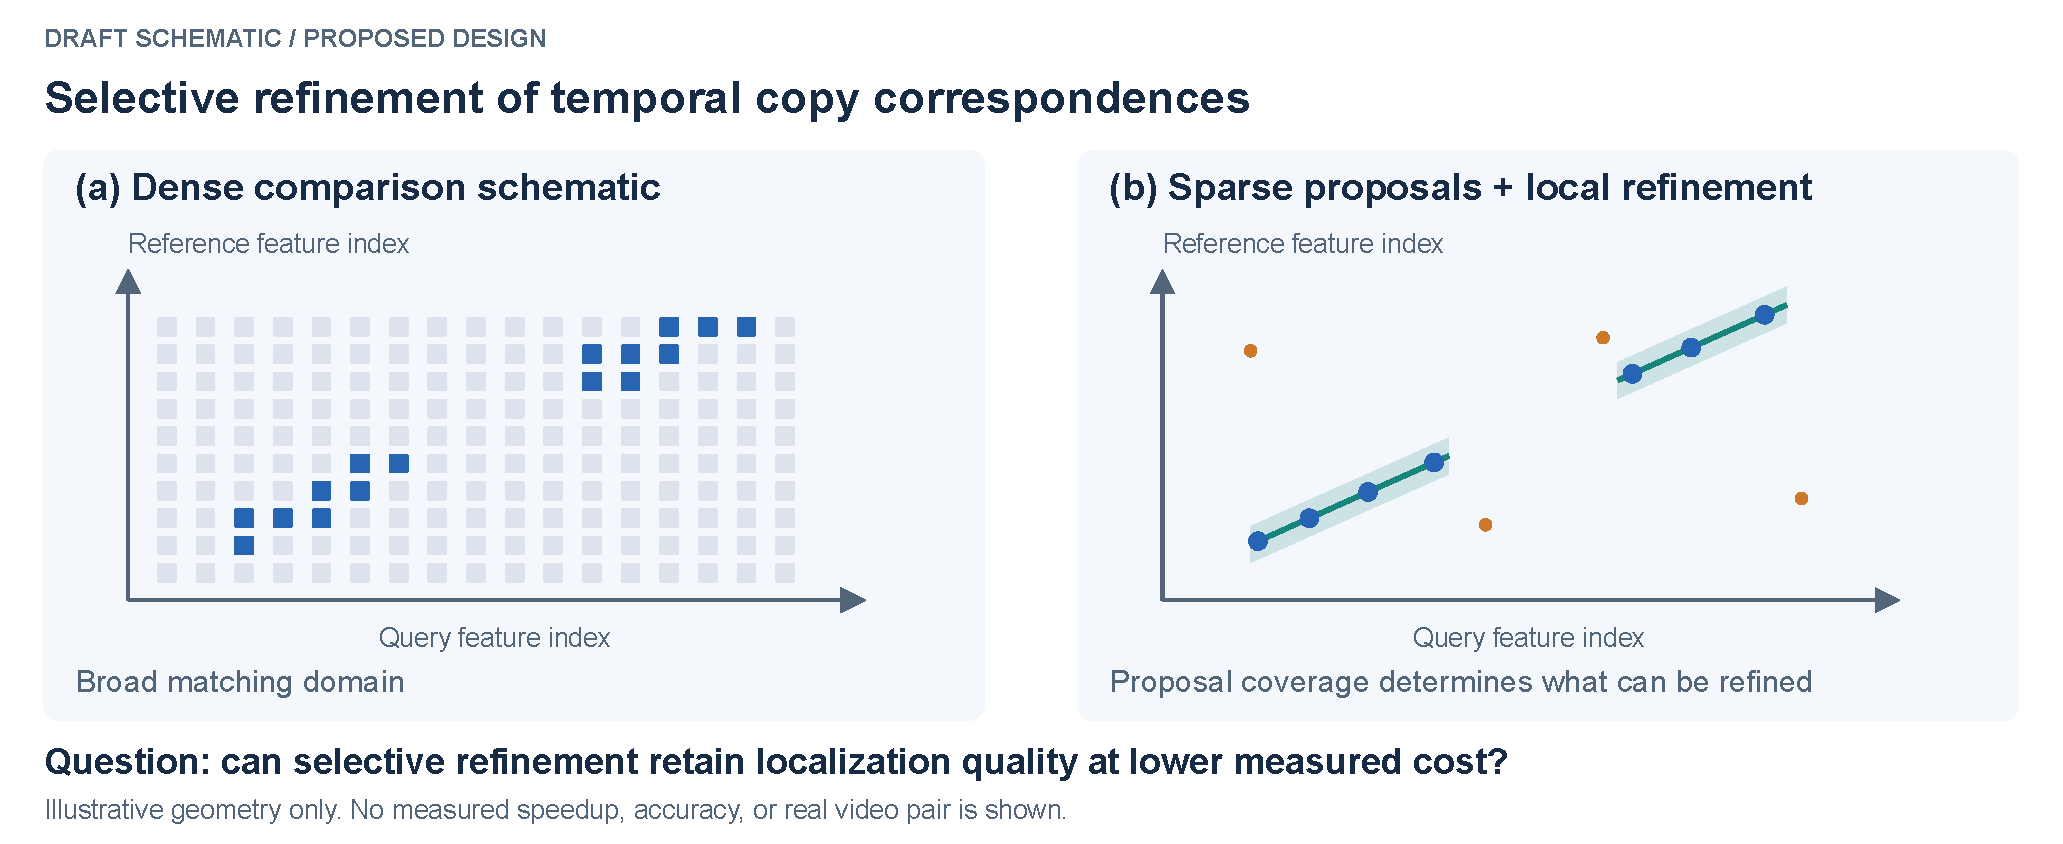
\includegraphics[width=\textwidth]{figures/fig_1_teaser.pdf}
  \caption{\textbf{Matching domains (conceptual schematic).}
  Sparse temporal proposals restrict fine alignment to finite regions. This hand-chosen
  geometry illustrates the hypothesis; it is not a benchmark result.}
  \label{fig:s-teaser}
\end{figure*}

\begin{figure*}[t]
  \centering
  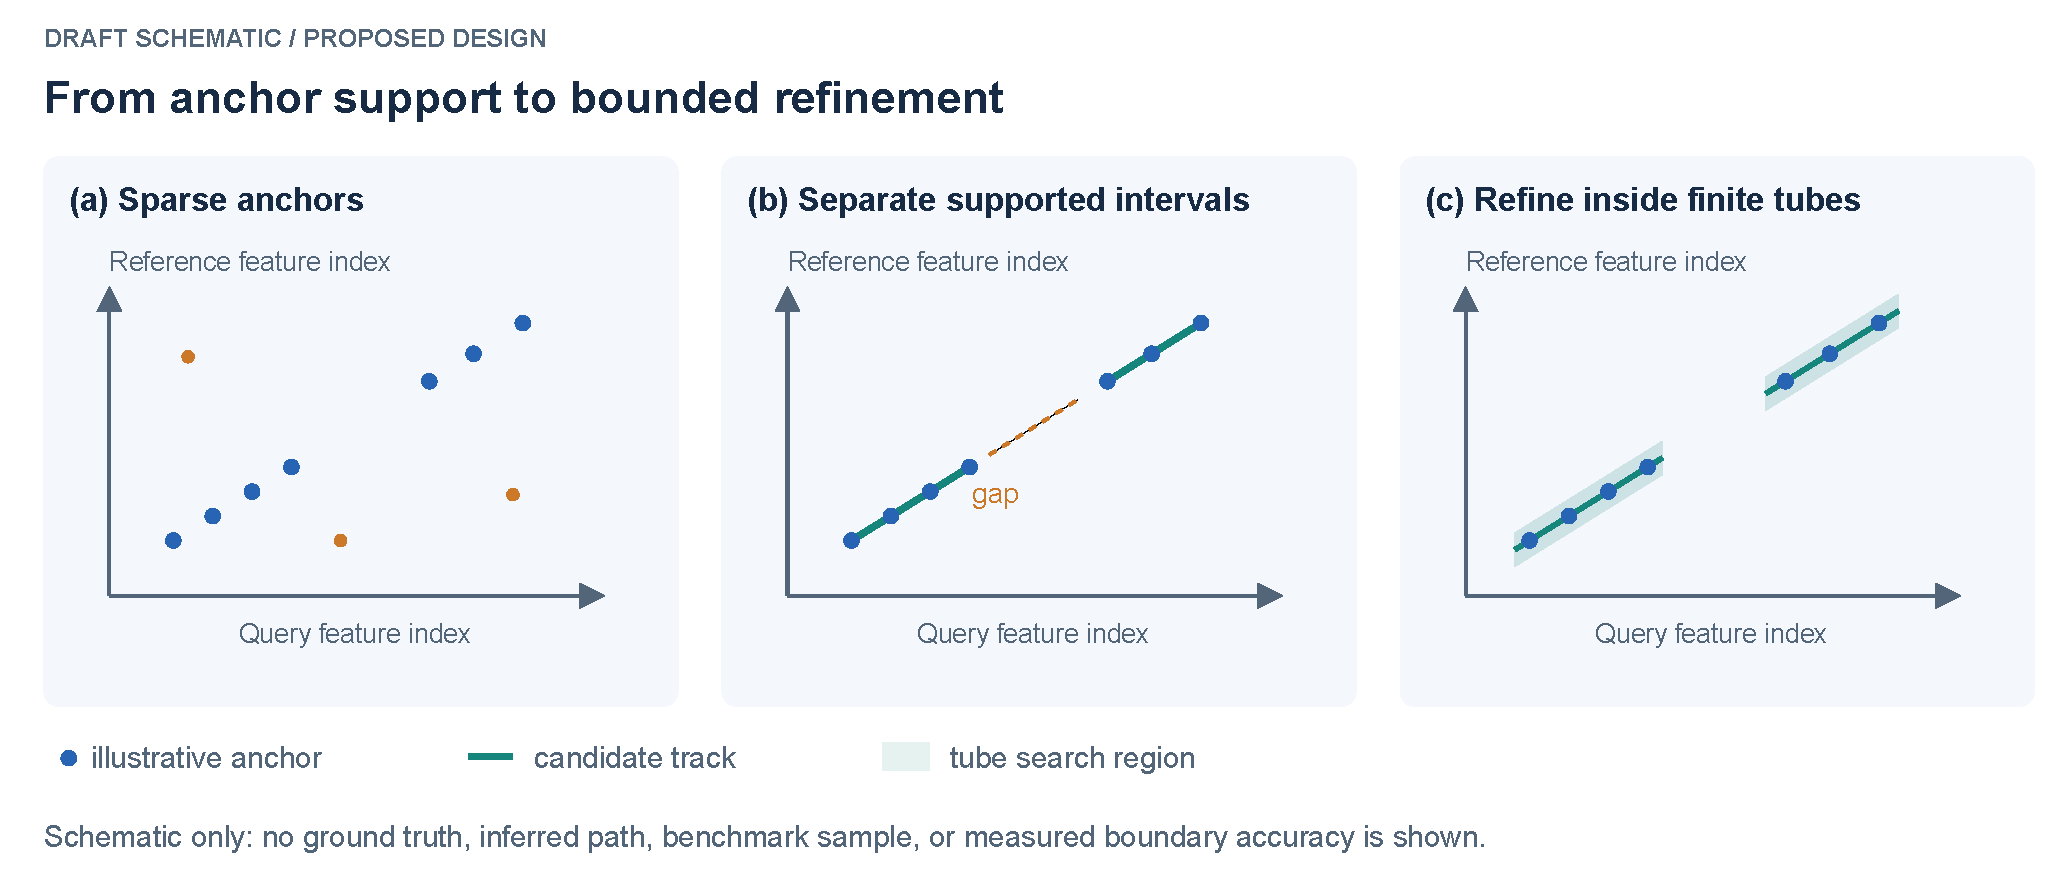
\includegraphics[width=\textwidth]{figures/fig_3_sparse_tracks.pdf}
  \caption{\textbf{From anchors to finite tubes (illustrative schematic).}
  (a) Sparse correspondences contain copy-supported and spurious anchors. (b) Inliers of a
  fitted track split at an unsupported gap. (c) Each interval defines a finite tube, and
  alignment is restricted to the shaded region. Coordinates are synthetic and hand-chosen;
  this is an algorithm illustration, \emph{not} a qualitative result on a real pair, and it
  contains no ground truth or measured boundary.}
  \label{fig:s-sparse-tracks}
\end{figure*}

\section{Implementation audit: deviations and consequences}
\label{sec:s-impl}

The main paper specifies the method; this section records where the current reference
implementation differs, so that a later reader does not mistake a prototype for the
specification.

\subsection{Local DP restart semantics}
\label{sec:s-dp}

The proposed recurrence is the zero-floored local-alignment equation in the main Method. The reference
implementation initializes a cell with no legal predecessor at $\max(0,r_{ij})$, but a cell
with a legal predecessor receives the continuation value \emph{unconditionally}, even when
that value is negative. Its documentation defends this as treating a weak frame as weak
evidence rather than as the absence of evidence. The two readings agree whenever all
evidence is strong. They differ in two regimes, which are the reason the choice is an
experimental variable:

\begin{table}[h]
\centering
\caption{Deterministic hand-constructed bands (one column). Both use
$\tau_{\mathrm{align}}=0.6$, $\lambda_{\mathrm{gap}}=0.1$, step set $\{(1,1)\}$. These are
scalar recurrence checks, not benchmark results. Copy cosine is 0.95, weak cosine is 0.0;
row $i$ contains only the match cell $(i,i)$.}
\label{tab:s-dp}
\footnotesize
\setlength{\tabcolsep}{3pt}
\resizebox{\columnwidth}{!}{%
\begin{tabular}{@{}l c c@{}}
\toprule
Input & Zero-floored (proposed) & Continuation (prototype) \\
\midrule
10 weak + 5 copy & max $1.75$, path found & max $0$, unreachable \\
strong, weak, strong & $H=[0.35,0,0.35]$ & $H=[0.35,-0.15,0.20]$ \\
two copies, 7-frame gap & second block $0.35\ldots1.75$ & second block negative \\
\quad(first copy blocked) & & unreachable \\
\bottomrule
\end{tabular}}
\end{table}

The mechanism is not only the sign of the continuation. When a legal predecessor exists,
the prototype sets $H=\mathrm{own}+\max_{\mathrm{pred}}(H_{\mathrm{pred}}-\lambda g)$ and
never compares with $\max(0,\mathrm{own})$; it also lets a negative $H$ cell serve as a
predecessor. A negative cell cannot start a traceback (its backpointer is cleared), but it
can be the first node of a later path and force a strong frame to pay the deficit. The
proposed recurrence restarts at the current cell and accepts only predecessors with $H>0$.

In the first input, the prototype's accumulated score after the weak prefix is negative at
every copy row, so the global maximum is 0 and no prediction is produced. In the second
input, the prototype finds the first block; after blocking its path, the second block is
still reached only through the unblocked weak gap and remains negative, so the second copy is
lost. The zero-floored recurrence restarts at the first copy row (case 1) and at the second
copy block (case 2). The mirror risk also exists: with a very short accumulated score, a
single weak frame can trigger an early restart. The zero floor is therefore not universally
better; E3 measures both on real candidates.

The existing unit test named ``restarts after a negative run'' does not distinguish the two
semantics: its global maximum lies in the first positive block, so both implementations pass
while the second block remains negative. Two further diagnostics are required before the
default is fixed: a long weak prefix followed by a true copy, and two same-track copies with
a long weak gap at the DP layer.

\subsection{Validity threshold, finite rows and the RANSAC draw}
\label{sec:s-valid}

The main text uses $\varepsilon=10^{-8}$; the prototype's shared constant is also $10^{-8}$
(\texttt{MIN\_ROW\_NORM}), used by the sparse search and the tube. Segment extraction
consumes the resulting node-valid mask. An
earlier draft wrote $10^{-12}$, which would have made rows with norms in
$(10^{-12},10^{-8}]$ valid on paper and invalid in code. The threshold is now aligned to the
implementation. Feature files are checked for non-finite values when loaded; the explicit
finite term in the mask keeps the definition safe for direct callers. The normalization
helper itself does not test \texttt{isfinite}: an \texttt{Inf} row has an infinite norm,
compares above the threshold, and divides to \texttt{NaN}. This is a helper-level gap to
harden before the helper is exposed as a public API; the pipeline itself rejects the file at
load.

The RANSAC draw is two anchors at distinct A coordinates. The code does not impose a minimum
A separation at draw time; the accepted run must still satisfy the A span
($L^A_{\min}=4$), the B span ($L^B_{\min}=8$) and the distinct-support minimum
($h_{\min}=5$). A minimum draw separation would be a new constraint, not a description of
the current algorithm.

\subsection{Predecessor addressing}
\label{sec:s-pred}

The ideal recurrence addresses the predecessor by its band-relative column
$\delta_u=(j-\Delta j)-c_r(i-\Delta i)$, which is $O(1)$ per step. The reference
implementation enumerates every column of the predecessor row for the non-diagonal steps and
filters by the actual index difference; that is $O(W_r)$ per cell and $O(P_rL_rW_r^2)$ per
tube. The two are reported separately in the complexity section and in E5. A wall-clock
number is only meaningful with the implementation named.

\subsection{Coarse-stage dot products}
\label{sec:s-dots}

The implementation performs a forward Top-$K$ scan, a backward Top-$K$ scan and, when ties
touch the $K$-th position, a re-scan of the tie group. The executed count is therefore close
to twice the one-direction grid size plus tie work. The efficiency comparisons use the
executed count, not the idealized one-pass count. The memory budget is a per-stage plan
computed before allocation; a budget violation is an explicit error, not a silent fallback.

\subsection{Sampling-plan interactions}
\label{sec:s-plan}

Multi-scale plans and non-default independent-phase plans are implemented, but their
combination is refused by the configuration rather than silently scanning the product. The
formal default is a single zero-phase stride-4 grid with Top-1 mutual matching. Multi-scale
must be compared with a single fine grid at the same dot-product budget; without that control,
a gain can be a budget increase rather than a scale effect.

\subsection{Segment post-processing}
\label{sec:s-seg}

A path is smoothed with a centered window of 3; cosines are clamped below zero before
edge-padded smoothing; nodes at or above $\tau_{\mathrm{seg}}=0.6$ are strong evidence. Runs
split when the number of intervening A indices exceeds $g_{\mathrm{low}}=2$ (equivalently the
index difference exceeds 3); weak leading/trailing nodes are trimmed; a run must reach 3
frames on A, 4 on B and contain two anchor entries. Two details are easy to misread. First,
\texttt{boundary\_margin} expands the strong span by that many \emph{matched path rows}
before endpoints are taken; it is not a feature-index margin, and on a local-DP path two rows
need not be two original A indices. The reference value is 2; the proposed Method uses zero
output margin. Second, the support count is over stored A-anchor entries in an A-only
interval, not distinct A times inside both intervals; with Top-$K>1$ the same A time can
contribute several entries. The proposed score uses the distinct-both-axes rule. These are
unresolved implementation differences, not completed fixes.

The prototype score is
$0.7\cdot\operatorname{clip}(\bar s,0,1)+0.3\cdot\min(1,N_{\mathrm{seg}}/
\max(1,L_A/\bar\Delta_A))$, where $N_{\mathrm{seg}}$ is the stored-entry count above. It is
not a learned objectness and is not calibrated against one. The prototype writes all
post-deduplication segments with scores; the confidence threshold is applied by the
evaluator (legacy mode: $q>c$, and $c=0$ skips both filtering and integer conversion). The
proposed Method should not be read as thresholding inside the core pipeline.

\subsection{A-range fallback when $e_A=0$}
\label{sec:s-arange}

The tube equation uses the A extension \(e_A\). In the code, \texttt{candidate\_a\_range}
pads by \texttt{half\_width + margin} when no explicit range is supplied, and the refinement
call supplies an explicit range only when \texttt{extension\_a>0}. With $w_r=12$ and margin
2, an $e_A=0$ run would therefore scan 14 extra A positions on each side rather than zero.
An E4 row that varies \(e_A\) must pass an explicit A range for the zero-extension point, or
it changes two factors. The formal configuration uses $e_A=16$, for which the code and the
equation agree.

\section{Metric details}
\label{sec:s-metric}

\paragraph{Product, not minimum.}
For a pair with predictions $P_k$ and GT $G_l$, the official per-pair precision is the
product of the two axis coverage ratios (the metric equation in the main Experiments). The union is taken over
the non-empty intersections of each prediction with all GT boxes, separately on each axis;
the denominator is the sum of the prediction lengths on that axis. Recall is symmetric. The
two-axis minimum is used only for de-duplicating our own predictions. A system that covers the
right query interval but the wrong reference interval receives a product near zero, which is
the intended behaviour.

\paragraph{Sentinel exclusion.}
The official dataset aggregate drops every per-pair value exactly equal to 1. The degenerate
cases are: empty prediction with non-empty GT ($P=1$ sentinel, $R=0$); non-empty prediction
with empty GT ($P=0$, $R=1$ sentinel); both empty ($P=R=1$). For nonempty inputs each axis denominator adds $10^{-6}$, so ordinary perfect overlap
scores slightly below 1 and is retained. For example, identical $10$ by $20$ intervals
give $(10/(10+10^{-6}))(20/(20+10^{-6}))\approx0.99999985$.
Equality filtering remains dtype-dependent and must follow the source evaluator. The implementation therefore reports
\texttt{excluded\_precision\_eq\_1} and \texttt{excluded\_recall\_eq\_1}, and we preserve the
behaviour for comparability instead of silently ``fixing'' it. A cleaned version would change
the numbers and must be a separate protocol, not a drop-in replacement.

\paragraph{Four denominators.}
For a run, print \texttt{n\_expected} (list size), \texttt{n\_processed}
(\textsc{ok}+\textsc{empty}), \texttt{n\_precision\_denom}=$|\{p:P_p\neq1\}|$ and
\texttt{n\_recall\_denom}=$|\{p:R_p\neq1\}|$. The last two are the true macro denominators;
record them directly from the evaluator; do not infer them from a directory name or
rounded metric values. Ordinary nonempty perfect matches are not sentinel cases. Also print \texttt{n\_pairs\_with\_gt},
\texttt{n\_pairs\_with\_pred}, \texttt{n\_pairs\_with\_gt\_and\_pred},
\texttt{n\_error}, \texttt{n\_skipped} and the threshold used. A run whose status file does
not account for every selected pair is not admissible.

\paragraph{Negative-pair FAR.}
The negative FAR is the fraction of the 27,315 key-missing test pairs with at least one
prediction. It is not defined on the validation split, which has no negatives. The official
macro mean is not a substitute: a correctly rejected negative pair has $P=R=1$ and is dropped
from both means, so correct rejections do not enter the reported F1 at all. This is why the
paper reports FAR separately.

\section{Evaluator parity check}
\label{sec:s-parity}

The port in \texttt{fastvcl/evaluate.py} was compared with the reference
\texttt{metric/eval.py} on synthetic boxes only. The check contains 11 hand-built cases
(identical, partial, disjoint, empty prediction, empty GT, both empty, multiple boxes,
overlapping predictions, touching intervals, float coordinates) and 200 deterministic random
cases with 0--3 predictions and 0--3 GT boxes.

Results:

\begin{itemize}
\item per-pair precision and recall: \textbf{211/211 exact}, maximum absolute difference
  $0.0$;
\item macro precision/recall and the exact-1 sentinel counts: identical on a synthetic
  result dictionary;
\item a five-row end-to-end accounting case: 4 scored pairs, 1 excluded \textsc{error},
  $|D_P|=|D_R|=2$, and two excluded exact-1 values per mean;
\item ordinary nonempty perfect overlap is retained at
  $0.9999998500000175$, not filtered as a sentinel;
\item the legacy \texttt{conf=0} branch performs neither score filtering nor integer
  truncation.
\end{itemize}

This is a \emph{function-level} parity result. It does not read the VCSL feature files, GT
JSON or a prediction file, and it does not certify the full evaluator entry point or the
official dataset score. The reference's bare \texttt{except: []} branch for malformed
predictions is deliberately not ported: the port refuses malformed input instead of
converting it to an empty prediction, which is the safer accounting rule.

\section{Dataset composition and GT anomalies}
\label{sec:s-data}

The local VCSL copy has 12,254 feature files (4,388,241,152 bytes), 97,033 training pairs,
41,798 validation pairs and 54,630 test pairs. Validation is 100\% positive; the test split
contains 27,315 key-missing pairs, treated as negatives. The CSV hashes are
\texttt{f7065467\ldots} (val), \texttt{b52c1b5f\ldots} (test) and
\texttt{47d492e2\ldots} (labels). Feature lengths range from 3 to 12,590 rows.

GT anomalies are kept, counted and never used to adjust candidates or predictions. In
validation, 60 intervals in 59 pairs extend beyond the feature length (maximum excess 108
indices) and 4 intervals are zero-length or reversed. In test, 8 intervals are out of range
and 45 are degenerate. A cleaned-subset analysis, if performed, must be frozen separately and
must not be presented as the official metric. The old data shipped next to a reference
implementation (55,530 pairs, 27,765 keys) is a different release and must not be mixed with
these files.

\section{Protocol details}
\label{sec:s-protocol}

\paragraph{Iso-budget comparison (E2).}
The budget is the executed number of dot products, not a nominal stride. For a zero-phase grid of stride $s$ with all rows valid, the one-direction count is
$\lceil M/s\rceil\lceil N/s\rceil$; the executed count
including the two directions and tie passes is read from the run log. A multi-scale or
multi-phase configuration is compared with a single fine grid whose executed count matches it
within a pre-declared tolerance. Exact equality may be unavailable for discrete grids;
in that case report the realized budgets without an iso-budget claim. For $M=N=64$,
stride 2 scores 1,024 grid pairs, while $\{2,4,8\}$ scores 1,344 before directional
rescans. Candidate recall and latency are plotted against executed count.

\paragraph{Single-factor rows (E4).}
Each row changes one item relative to the reference configuration. The RANSAC seed is derived
from the global seed and the pair id, so reruns are identical. The headline rows are repeated
with five seeds; the standard deviation is reported. A ``no geometry'' row is implemented as
a local-window proposal around the highest-scoring anchor clusters at the same dot-product
budget, never as ``skip fitting and output zero predictions''.

\paragraph{Timing (E5).}
Start: raw features resident in CPU memory, operators initialized. End: five-column
predictions exist in memory. Included: normalization, masking, tiling, transfers, sparse
matching, RANSAC, tube construction, band similarity, DP, traceback, post-processing and
in-memory serialization. Excluded and reported separately: feature file I/O, result export,
process initialization, video decoding and ISC extraction. Warm-up at least once, then at
least three measured rounds; profiling off; GPU timing synchronized at both ends; CPU threads
and GPU model reported.

\paragraph{TransVCL chunk timing.}
Measure all chunk pairs and assembly within the video-pair wall boundary, then compute
mean/P50/P95 over video pairs. A sum of model-forward times alone excludes preprocessing,
transfers or assembly and is not the primary pair latency.
Report the number of chunk pairs and the maximum chunk size. A single-chunk time is not a
video-pair time.

\section{Required log schema}
\label{sec:s-log}

Future runs should emit the following fields (null when unavailable, never invented):
\begin{itemize}
\item \texttt{run\_metadata.json}: run id, method, code commit, dirty-diff hash, config hash,
dataset version, split, CSV/GT/feature-manifest hashes, evaluator entry point,
\texttt{coordinate\_convention}, frozen protocol id, seed, hardware, backend, precision,
\texttt{timing\_scope}, \texttt{profiling\_enabled=false}.
\item \texttt{predictions.json}: pair id $\rightarrow$ list of
$[a_s,b_s,a_e,b_e,\text{score}]$.
\item \texttt{status.jsonl}: pair id, status (\textsc{ok}/\textsc{empty}/\textsc{error}/
\textsc{skipped}), reason, $M$, $N$.
\item \texttt{metrics.json}: split, \texttt{n\_expected}, \texttt{n\_processed},
\texttt{n\_error\_or\_skipped}, \texttt{n\_precision\_denom}, \texttt{n\_recall\_denom},
\texttt{n\_negative\_pairs}, precision, recall, f1, \texttt{negative\_pair\_far} (null on
validation), confidence threshold, \texttt{threshold\_selected\_on}, protocol id.
\item \texttt{per\_pair\_timing.jsonl}: pair id, repeat, warm-up flag,
\texttt{t\_localize\_ms}, \texttt{t\_io\_ms}, \texttt{t\_export\_ms}, stage times,
\texttt{actual\_dot\_products}, \texttt{tube\_cells\_evaluated}, number of tubes, CPU RSS,
GPU peak allocated/reserved, status.
\end{itemize}

\section{Efficiency and ablation matrices (reserved)}
\label{sec:s-matrices}

These matrices are moved out of the main text to keep the fallback page budget; they are not
additional results. Every cell is pending. The main Table~1 remains the primary comparison.

\begin{table*}[t]
\centering
\caption{\textbf{System efficiency, memory and stage breakdown.}
Same machine, feature files and protocol; per-tile profiling off; one warm-up and at least
three measured rounds. $\Tloc$ covers normalisation through in-memory prediction and excludes
feature I/O, export and video decoding. TransVCL timing includes all chunk pairs and pair-level
assembly. CPU-only methods report \texttt{N/A} for GPU memory. \TODO{All entries are pending.}}
\label{tab:s-efficiency}
\scriptsize
\setlength{\tabcolsep}{3pt}
\begin{tabular}{@{}l l c c c c c@{}}
\toprule
Method & HW & Pairs & $\Tloc$ mean/P50/P95 & Thr. & RSS/VRAM & F1 \\
\midrule
HV       & CPU & -- / 41{,}798 & -- / -- / -- & -- & -- / N/A & -- \\
TN       & CPU & -- / 41{,}798 & -- / -- / -- & -- & -- / N/A & -- \\
DP       & CPU & -- / 41{,}798 & -- / -- / -- & -- & -- / N/A & -- \\
DTW      & CPU & -- / 41{,}798 & -- / -- / -- & -- & -- / N/A & -- \\
TransVCL & GPU & -- / 41{,}798 & -- / -- / -- & -- & -- / -- & -- \\
Simple Sparse-to-Band & CPU & -- / 41{,}798 & -- / -- / -- & -- & -- / N/A & -- \\
FastVCL (proposed) & CPU & -- / 41{,}798 & -- / -- / -- & -- & -- / N/A & -- \\
FastVCL (CUDA path) & GPU & -- / 41{,}798 & -- / -- / -- & -- & -- / -- & -- \\
\bottomrule
\end{tabular}
\vspace{3pt}
\par\raggedright\footnotesize
Exact CPU/GPU models, thread counts and precision are pending. ``Pairs'' means
processed/expected validation pairs; report errors and skips separately. The CUDA row exists
only after real-hardware acceptance; until then \TODO{no GPU kernel has executed}.
\end{table*}

\begin{table*}[t]
\centering
\caption{\textbf{Controlled mechanism and hypothesis ablations (H1--H3).}
E1 includes a full-system comparison; E2--E4 name individual changes. ``Dots'' is the
executed dot-product count (both Top-$K$ directions and tie passes); ``cells'' reports
executed DP visits; log similarity dot products separately. Candidate recall and boundary
MAE are custom diagnostics, not the official metric. \TODO{All entries are pending.}}
\label{tab:s-ablation}
\scriptsize
\setlength{\tabcolsep}{3pt}
\renewcommand{\arraystretch}{1.02}
\begin{tabular}{@{}l l l c c c c c c@{}}
\toprule
Exp & Variant & Change & Dots & Cells & Cand.R & Bnd.MAE & F1 & Tloc \\
\midrule
E1 & Simple STB & reference & -- & -- & -- & -- & -- & -- \\
E1 & FastVCL core & full configuration & -- & -- & -- & -- & -- & -- \\
\midrule
E2 & stride 2 & $s=2$ & -- & -- & -- & -- & -- & -- \\
E2 & stride 4 & $s=4$ & -- & -- & -- & -- & -- & -- \\
E2 & multi-scale & add $\{2,8\}$ & -- & -- & -- & -- & -- & -- \\
E2 & no de-dup & drop dedup & -- & -- & -- & -- & -- & -- \\
E2 & indep.\ phases & add offsets & -- & -- & -- & -- & -- & -- \\
\midrule
E3 & coarse support box & no refinement & -- & -- & -- & -- & -- & -- \\
E3 & band DTW & global & -- & -- & -- & -- & -- & -- \\
E3 & continuation & prototype & -- & -- & -- & -- & -- & -- \\
E3 & zero-floored DP & proposed recurrence & -- & -- & -- & -- & -- & -- \\
\midrule
E4 & no support & support/span off & -- & -- & -- & -- & -- & -- \\
E4 & no split & one run/line & -- & -- & -- & -- & -- & -- \\
E4 & joint IoU & replace min-IoU & -- & -- & -- & -- & -- & -- \\
E4 & extension & vary $e_A$ only & -- & -- & -- & -- & -- & -- \\
E4 & half-width & vary $w_r$ only & -- & -- & -- & -- & -- & -- \\
\midrule
E5 & scan & prototype & -- & -- & -- & -- & -- & -- \\
E5 & offset & $O(LW)$ & -- & -- & -- & -- & -- & -- \\
\bottomrule
\end{tabular}
\vspace{3pt}
\par\raggedright\footnotesize
Rows are grouped by experiment; within E2--E4 only the named factor changes. Multi-scale rows
need a single-grid control matched by executed work; stride 2 is not automatically
equal-budget to $\{2,4,8\}$. RANSAC seed is fixed per pair; headline rows are repeated over
five seeds. The zero-extension E4 row must pass an explicit A range (Section~\ref{sec:s-arange}).
\end{table*}

\begin{figure}[t]
  \centering
  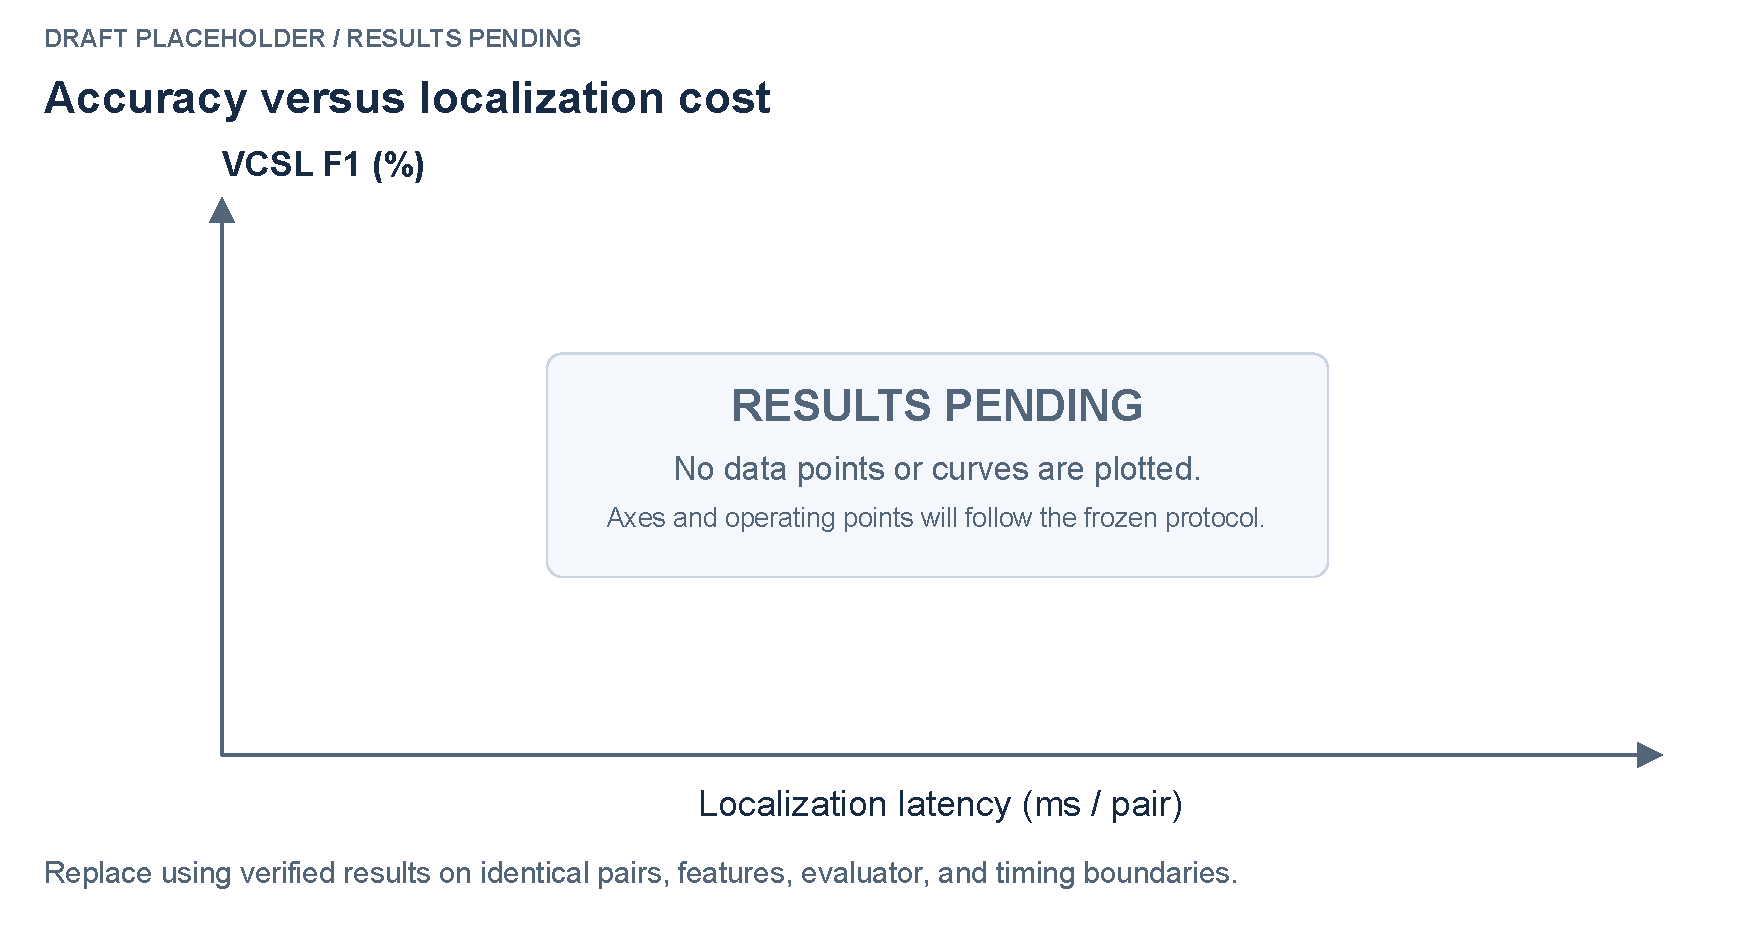
\includegraphics[width=\columnwidth]{figures/fig_4_tradeoff.pdf}
  \caption{\textbf{Reserved quality--cost plane (results pending).}
  No points or fitted curves are shown. Future points require measured pair-level latency,
  frozen configurations and one common evaluator.}
  \label{fig:s-tradeoff}
\end{figure}

\section{Status of the existing development runs}
\label{sec:s-status}

The following are recorded so that no later reader mistakes them for benchmark results. They
are \textsc{pilot-only}.
\begin{itemize}
\item A validation run that finished 8,075 of 41,798 pairs (5,873 \textsc{ok}, 2,202
\textsc{empty}, 0 error, 33,723 skipped) because it was interrupted.
\item A near-complete validation run that attempted all 41,798 pairs: 28,708 \textsc{ok},
13,089 \textsc{empty}, 1 error; the metrics file scores 41,797 pairs. It is not a zero-error
evaluation and its configuration is not a frozen protocol.
\item A 1,000-row development list whose metrics file is computed over 200 scored pairs; the
directory name and its \texttt{COMPLETE} label are not a sample-size claim.
\item A 24-pair synthetic run and several 20-pair real development runs. Synthetic numbers
are never used as real-data results, and 20-pair numbers carry no statistical claim.
\item A CUDA implementation that has never executed on a GPU; all GPU-related conclusions
are \textsc{missing}, not zero.
\end{itemize}

\section{Reproduction checklist}
\label{sec:s-repro}

Before any number enters the main tables: (1) freeze the feature content digest, pair CSV,
GT and evaluator; (2) select each method's threshold on validation and freeze it; (3) run
validation to zero errors; (4) run test once; (5) fill the four denominators; (6) repeat the
timing with profiling off and at least three rounds; (7) archive the run id and config hash;
(8) only then replace the \TODO{PENDING} cells. Until step (8), the main paper must keep the
placeholders visible.


\section{Round-two design corrections and optional E6}
\label{sec:s-round2}
\paragraph{Baseline controls.}
The simple sparse-to-band baseline shares the grid, coarse matcher, RANSAC trial cap,
fixed tube width/extension, zero-floored step set, scoring and min-IoU output rule with the
core method. It omits the extra dual-axis support/span checks and gap splitting, and uses
one path per tube. Its inlier minimum still requires sufficient distinct A times for a line.
E1 matches configured caps and executed coarse work, not realized candidate counts.
E3 alone reuses identical serialized tracks/tubes, with hashes, for refinement comparisons.
Full-matrix DP changes the search domain and is not an indexing-only ablation.

\paragraph{Sampling bound and uncertainty.}
The lower bound $(h-1)s+1$ applies to the span of $h$ distinct anchors on one stride-$s$
grid. A short copy cannot supply that many internal anchor times, but outside anchors and
tube extension can still overlap it. It is not a universal no-detection theorem. Likewise,
gap splitting followed by validation can reduce the number of accepted tracks to zero.
For matched-boundary analysis report conditional MAE, matched counts, recall and the common
GT cohort across methods. Five RANSAC seeds measure fitting variability only. A paired
bootstrap needs a declared sampling unit and treatment of shared-video dependence; if this
cannot be justified, report descriptive variation without a significance claim.

\paragraph{E6: selective visual verification (proposed, not run).}
The \texttt{seltive model} branch uses original frames, a verified timestamp/index map,
a frozen model/checkpoint or API version, and a frozen prompt/output schema. On a fixed
candidate pool compare: core only; uniform random selection; a cheap declared selection
rule; and the proposed selective rule. Match call/frame/token budgets and repeat selection
seeds. Report correction of false candidates, rejection of true candidates, unchanged cases,
uncertain/failed calls, full-set F1/recall/FAR and total added latency/cost. Metrics on selected
candidates alone are insufficient. A verifier-oracle score, if used, is an analysis ceiling,
never a deployed policy. No GT may select candidates at inference.

Frame reading/decoding, model preprocessing, queue/network time, retries and fusion belong
in the extension cost. Cached evidence and live acquisition are separate settings. Unselected,
uncertain and failed cases retain the core result; decisive-verdict fusion is still an open
design. E6 requires independent negative calibration data if the selection/fusion policy is
tuned for false alarms; the positive-only validation split cannot supply that evidence.

\paragraph{Verification scope (round 3).}
Three read-only checks were run. (i) The prototype's unit suite: 646 tests, 0 failures,
10 CUDA tests skipped because no GPU executed. (ii) Evaluator parity: 211 synthetic cases,
zero per-pair mismatch, identical macro and sentinel counts, and a five-row status/accounting
case (Section~\ref{sec:s-parity}). (iii) Eight contract probes on hand-built bands: weak
prefix, strong--weak--strong, two copies after blocking, invalid cells, A-range fallback,
ties-to-even rounding, margin 0/2, duplicate-versus-distinct support and the segment gap
boundary. These are semantics and accounting checks, not benchmark results. They do not
execute a VCSL pair, a model checkpoint or a GPU kernel, and they do not certify an
end-to-end evaluator file run. The proposed zero-floor recurrence, distinct support, zero
margin and pipeline-side threshold remain unimplemented; the prototype continuation and the
stored-entry support are the current behaviour.

\end{document}
